\hypertarget{what-the-data-say-pre-registered-audits}{%
\section{What the data say: pre-registered
audits}\label{what-the-data-say-pre-registered-audits}}

The preceding sections worked in model units. This section turns to
public data, and asks only questions that a calibrated audit can answer.
The audits test whether fitted corrections to the homogeneous expansion
are consistent across declared model families and data splits
\citep{TsiokosDarkEnergy2026}. Either outcome alone leaves the physical
origin of the constant term unresolved: subset dependence can also arise
from noise, fitting choices or unmodeled systematics.

The data are DESI DR2 BAO \citep{DESI2025DR2}, Pantheon+ supernova
distances \citep{Brout2022} and compressed Planck distance priors,
analysed with a compressed likelihood pipeline in which the supernova
intercept is profiled analytically. The statistics, splits and
thresholds were pre-registered before the audit tables were generated,
using data products and baseline fits from an earlier stage of the
program (Section 3.4); the amendments are listed there and in Appendix
B.

\hypertarget{a-rewrite-family-is-constant-compatible}{%
\subsection{A rewrite family is
constant-compatible}\label{a-rewrite-family-is-constant-compatible}}

Three models were fitted with the same likelihood and nuisance treatment
to \(n=1604\) data points:

\begin{longtable}[]{@{}llllll@{}}
\toprule
\begin{minipage}[b]{0.29\columnwidth}\raggedright
model\strut
\end{minipage} & \begin{minipage}[b]{0.04\columnwidth}\raggedright
\(k\)\strut
\end{minipage} & \begin{minipage}[b]{0.11\columnwidth}\raggedright
\(\chi^2\)\strut
\end{minipage} & \begin{minipage}[b]{0.10\columnwidth}\raggedright
\(\Delta\)AIC\strut
\end{minipage} & \begin{minipage}[b]{0.10\columnwidth}\raggedright
\(\Delta\)BIC\strut
\end{minipage} & \begin{minipage}[b]{0.20\columnwidth}\raggedright
parameters\strut
\end{minipage}\tabularnewline
\midrule
\endhead
\begin{minipage}[t]{0.29\columnwidth}\raggedright
\(\Lambda\)CDM\strut
\end{minipage} & \begin{minipage}[t]{0.04\columnwidth}\raggedright
4\strut
\end{minipage} & \begin{minipage}[t]{0.11\columnwidth}\raggedright
1455.80\strut
\end{minipage} & \begin{minipage}[t]{0.10\columnwidth}\raggedright
0\strut
\end{minipage} & \begin{minipage}[t]{0.10\columnwidth}\raggedright
0\strut
\end{minipage} & \begin{minipage}[t]{0.20\columnwidth}\raggedright
\(\Omega_m=0.303\)\strut
\end{minipage}\tabularnewline
\begin{minipage}[t]{0.29\columnwidth}\raggedright
\(w_0w_a\)CDM\strut
\end{minipage} & \begin{minipage}[t]{0.04\columnwidth}\raggedright
6\strut
\end{minipage} & \begin{minipage}[t]{0.11\columnwidth}\raggedright
1442.17\strut
\end{minipage} & \begin{minipage}[t]{0.10\columnwidth}\raggedright
\(-9.63\)\strut
\end{minipage} & \begin{minipage}[t]{0.10\columnwidth}\raggedright
\(+1.13\)\strut
\end{minipage} & \begin{minipage}[t]{0.20\columnwidth}\raggedright
\(w_0=-0.795\), \(w_a=-0.673\)\strut
\end{minipage}\tabularnewline
\begin{minipage}[t]{0.29\columnwidth}\raggedright
rewrite, \(E^2=\Omega_m(1+z)^3+\Omega_r(1+z)^4+A(1+z)^m\)\strut
\end{minipage} & \begin{minipage}[t]{0.04\columnwidth}\raggedright
6\strut
\end{minipage} & \begin{minipage}[t]{0.11\columnwidth}\raggedright
1453.66\strut
\end{minipage} & \begin{minipage}[t]{0.10\columnwidth}\raggedright
\(+1.85\)\strut
\end{minipage} & \begin{minipage}[t]{0.10\columnwidth}\raggedright
\(+12.61\)\strut
\end{minipage} & \begin{minipage}[t]{0.20\columnwidth}\raggedright
\(A=0.699\), \(m=0.068\) (best fit)\strut
\end{minipage}\tabularnewline
\bottomrule
\end{longtable}
\addtocounter{table}{-1}

The \(w_0w_a\) comparison \citep{ChevallierPolarski2001, Linder2003}
reproduces the familiar survey-era picture: a preference by AIC that BIC
does not share \citep{Liddle2007}. The rewrite family tests whether the
correction the data prefer depends on redshift. Its shape parameter is
compatible with a constant under the pre-registered criterion
\(|m|\le\min(2\sigma_m,0.25)\), with best fit \(m=0.068\) and
\(\sigma_m=0.074\); the posterior median is \(m=0.131\), with 16th and
84th percentiles \(0.057\) and \(0.204\). The rewrite also pays an Occam
penalty relative to \(\Lambda\)CDM. On these data and this pipeline,
then, the fitted correction is consistent with a constant. This says
that current geometry does not separate this rewrite family from its
constant member; it does not explain why \(\Lambda\)CDM fits, and it
does not distinguish a fundamental constant from an effective one.

\hypertarget{one-expansion-history-two-descriptions}{%
\subsection{One expansion history, two
descriptions}\label{one-expansion-history-two-descriptions}}

A canonical scalar field with a standard two-derivative action and
positive energy density cannot reach \(w<-1\) without a wrong-sign
kinetic term \citep{Caldwell2002, Vikman2005}, so a preference for
crossing \(w=-1\) is often read as a problem. The same expansion history
can also be written as an additive correction to the
matter-plus-radiation expansion rate,
\(\Delta_H(z)=E^2_{w_0w_a}(z)-\Omega_m(1+z)^3-\Omega_r(1+z)^4\) with
\(E=H/H_0\), which does not by itself specify a microscopic fluid model.

For the CPL form \(w(z)=w_0+w_az/(1+z)\), the dark-energy contribution
to \(E^2\) is
\[\rho(z)=\rho_0(1+z)^{3(1+w_0+w_a)}\exp\!\Bigl(-\frac{3w_az}{1+z}\Bigr),\qquad
\rho'(z)=\frac{3\,\rho(z)\,\bigl(1+w(z)\bigr)}{1+z}.\] For \(\rho_0>0\)
and \(z>-1\), \(\rho\) is positive and smooth, the additive correction
\(\Delta_H\) equals \(\rho\), and, with nonnegative matter and radiation
coefficients, \(E^2>0\). The equation of state reconstructed from the
logarithmic derivative of \(\Delta_H\) is the same \(w(z)\), with the
same crossing. The density is stationary exactly where \(w=-1\), and
when \(1+w_0+w_a\ne0\) this happens only at
\(z_\star=-(1+w_0)/(1+w_0+w_a)\). These identities are mechanized. For
the best-fit parameters of Section 8.1, \(z_\star=0.4388\); in the
additive description the crossing is simply the maximum of a smooth
positive density, which ranges from \(0.499\) to \(0.760\) over
\(0\le z\le2.5\) (Figure \ref{fig:audits}a).

The two descriptions are mathematically equivalent ways of writing the
same history. A preference for crossing is therefore a statement about
the fitted history, and its interpretation depends on which description
is taken as physical. The calculation does not show that ghosts are
absent from any physical model, and it does not show that dark energy is
not a fluid.

\hypertarget{the-staging-audit-flags-supernovabao-subset-dependence}{%
\subsection{The staging audit flags supernova--BAO subset
dependence}\label{the-staging-audit-flags-supernovabao-subset-dependence}}

\textbf{Statistic.} The rewrite shape is refitted on declared splits of
the data (BAO only, supernovae only, and supernovae below and above
\(z=0.35\)), and the audit records the largest standardized shift from
the joint fit,
\[S=\max_{\rm split}\frac{|m_{\rm split}-m_{\rm joint}|}{\sqrt{\sigma^2_{\rm split}+\sigma^2_{\rm joint}+0.05^2}} .\]
The staging fits use a reduced vector of thirteen BAO points and six
compressed supernova summaries, with the matter density fixed at a value
taken from the earlier fit to the observed data; Planck is not included.

\textbf{Calibration.} Twenty mock \(\Lambda\)CDM realizations through
the identical pipeline set the threshold. With twenty mocks and a
nominal level of \(1/20\), the conservative rank rule rejects only above
the largest mock score, \(8.879\). If the observed and mock scores were
exchangeable, this rule would bound the false-alarm probability by
\(1/21\); because the mocks are generated at parameters fitted to the
observed data, that premise is not established, and the rank fraction is
descriptive. (The originally declared interpolated 95th percentile was
\(8.328\).)

\textbf{Power.} The originally declared alternatives applied one rewrite
coherently to all probes and were never detected. A common shift of all
split estimates cancels in every term of \(S\) when the uncertainties
are unchanged, so such alternatives are expected to leave the rejection
rate at its null value rather than raise it. An audit of staging
dependence needs alternatives that break the symmetry the statistic
measures. Alternatives applied to one probe at a time do: a supernova
distance-modulus tilt \(\mu\to\mu+\varepsilon(z/0.5)\) was detected in
17 of 20 mocks at \(\varepsilon=0.20\), and a BAO tilt
\(\alpha\to\alpha(1+\varepsilon(z-0.8))\) in 20 of 20 at
\(\varepsilon=0.10\), the smallest tested amplitudes reaching a rate of
\(0.8\) (Figure \ref{fig:audits}b). With twenty mocks per amplitude
these rates are empirical, not population power.

\textbf{Verdict.} On the real data \(S=9.630\), above the cutoff (Figure
\ref{fig:audits}c). The largest shift comes from the high-redshift
supernova split, whose fit sits at the upper bound of the amplitude
range; the supernova-only and low-redshift supernova fits sit at the
lower bound of the shape range. Its size is comparable to the tested
supernova tilt at \(\varepsilon\approx0.2\). We read the result as
structured probe dependence, consistent with the known mild tension
between supernova and BAO distances in this reduced, fixed-anchor
pipeline; comparisons of the two kinds of distance are the subject of
distance-duality tests \citep{Etherington1933, BassettKunz2004}. Because
the threshold is not a guaranteed level, the result carries no
population-level significance, and it does not identify the physical
source of the dependence. It is not evidence for a closure mechanism and
it is not a statement about \(\Lambda\).

\begin{figure}[t]
\centering
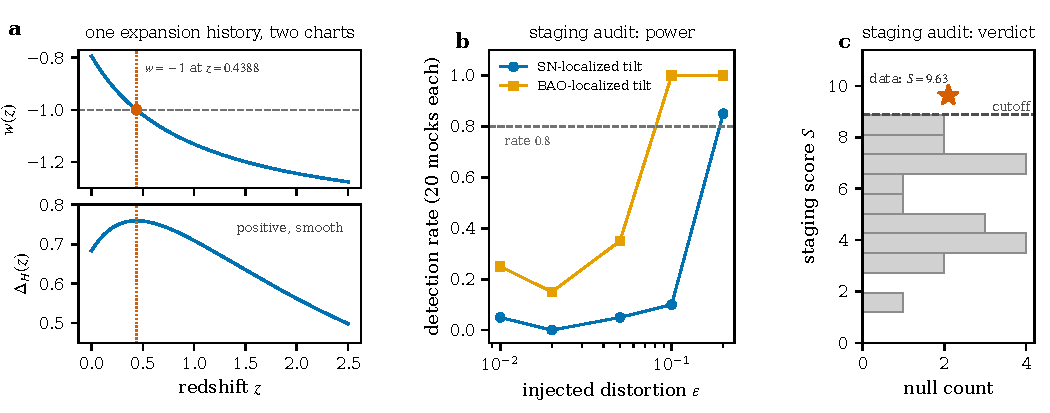
\includegraphics[width=\textwidth]{F6_audits.pdf}
\caption{\textbf{Real-data audits.} \emph{(a)} The best-fit $w_0w_a$ history in two descriptions: the fluid equation of
state $w(z)$ crosses $-1$ at $z_\star=0.4388$ (top), where the additive density $\Delta_H(z)$ has its maximum and stays
positive and smooth (bottom). \emph{(b)} Detection rates of the staging audit for probe-localized injections, from 20
mocks per amplitude, at the rank-rule cutoff. \emph{(c)} The 20 null scores, the cutoff (their maximum) and the observed
score.}
\label{fig:audits}
\end{figure}

\hypertarget{route-residuals}{%
\subsection{Route residuals}\label{route-residuals}}

The same reduced fits give unsigned residuals between routes: the
rewrite amplitude differs between the supernova-only and joint fits by
\(0.417\) and between the BAO-only and joint fits by \(0.116\); the
matter-density residuals are zero because that parameter is held fixed.
This demonstrates the protocol on the routes the data allow and inherits
the calibration status of Section 8.3. It does not address the \(H_0\)
tension, which needs distance-ladder data outside this battery.

\hypertarget{the-growth-data-cannot-yet-host-the-decisive-test}{%
\subsection{The growth data cannot yet host the decisive
test}\label{the-growth-data-cannot-yet-host-the-decisive-test}}

Structure growth is where a closure correction would be most
distinctive. The audit used three public shear and lensing data sets:
KiDS-Legacy COSEBIs (126 points, S/N 28.6), HSC-Y3 Fourier-space cosmic
shear (170 points, S/N 37.4) and the combined ACT, SPT and Planck
CMB-lensing bandpowers (35 points, S/N 61.4). Each data set was cut into
shells and each shell classified by a heterogeneity proxy \(H\), the
weighted mean excess of the log nonlinear-to-linear power, as slack
(\(H\le0.05\)), mild or strong (\(H\ge0.3\)). The audit statistic for a
shell is the price
\(\pi=[\lambda_{\max}(\Xi/q^{\rm row}_{0.95})-\Omega]_+\) of its
adequacy residual, normalized by a null with the same number of rows and
the data covariance, and every null result had to be accompanied by a
successful detection of an injected signal. That requirement caught a
mis-scaled null normalizer during development.

Three findings follow.

\begin{enumerate}
\def\labelenumi{\arabic{enumi}.}
\tightlist
\item
  \textbf{Support.} The slack and strong regimes are measured by
  different probes. In the computed proxy values, KiDS shells are all
  mild (\(H\) from about \(0.088\) to \(0.172\)), HSC shells all strong
  (about \(0.477\) to \(1.911\)), and CMB lensing has two slack shells
  and one mild (largest \(H\approx0.144\)); full-shape clustering
  reaches about \(H\approx0.11\) at the scales treated as reliable. None
  of the surveyed probes spans slack and strong shells within one data
  set and covariance, so the planned within-family comparison computed
  no price.
\item
  \textbf{Model dependence.} Where a strong-regime residual can be
  measured, in HSC, its size depends on the theoretical model: with
  linear modeling the shell prices are \(8.3\), \(8.8\), \(16.5\) and
  \(10.6\), while with nonlinear modeling \citep{Takahashi2012}, with or
  without nuisance parameters, every point price is zero; some
  confidence intervals keep positive upper limits. These model
  comparisons use local linearizations around the HSC best fit,
  propagated to 256 posterior perturbations, rather than full nonlinear
  evaluations of every posterior draw, and the fitted inputs are not
  independent data. All stored injection checks pass: the nonlinear
  configurations detect a finite injected signal (price \(3.9\)), while
  in the linear configurations the injection adds effectively no signal
  and so does not demonstrate incremental sensitivity there. The
  residual is therefore sensitive to omitted nonlinearity; this is not a
  unique causal attribution.
\item
  \textbf{What a decisive test needs.} One data set with both slack and
  strong shells under a common covariance and validated nonlinear
  modeling. Surveys of the LSST, Euclid and Roman class are candidates;
  whether they meet these support and modeling conditions would still
  have to be shown.
\end{enumerate}

The CMB-lensing shells, analysed separately as a diagnostic, also give
zero point prices with a live injection.
